\documentclass[12pt,a4paper]{article}
\usepackage[utf8]{inputenc}
\usepackage{graphicx}
\usepackage{geometry}
\usepackage{float}
\usepackage{hyperref}
\usepackage{listings}
\usepackage{color}

\geometry{margin=1in}

\definecolor{codegreen}{rgb}{0,0.6,0}
\definecolor{codegray}{rgb}{0.5,0.5,0.5}
\definecolor{codepurple}{rgb}{0.58,0,0.82}
\definecolor{backcolour}{rgb}{0.95,0.95,0.92}

\lstdefinestyle{mystyle}{
    backgroundcolor=\color{backcolour},   
    commentstyle=\color{codegreen},
    keywordstyle=\color{magenta},
    numberstyle=\tiny\color{codegray},
    stringstyle=\color{codepurple},
    basicstyle=\ttfamily\footnotesize,
    breakatwhitespace=false,         
    breaklines=true,                 
    captionpos=b,                    
    keepspaces=true,                 
    numbers=left,                    
    numbersep=5pt,                  
    showspaces=false,                
    showstringspaces=false,
    showtabs=false,                  
    tabsize=2
}
\lstset{style=mystyle}

\title{\textbf{Lab 4 - Logic Equivalence Check (LEC)}}
\author{Your Name / Roll No.}
\date{\today}

\begin{document}

\maketitle

\section*{Objective}
To understand the basics of Conformal LEC setup, and debug basic non-equivalences for the Sequential Multiplier design.

\section*{Task 1: LEC for Sequential Multiplier System}
\subsection*{Objective}
Perform a standard Logic Equivalence Check between the original RTL and the synthesized gate-level netlist to confirm that the synthesis tool correctly mapped the logic.

\subsection*{Implementation}
The setup script (\texttt{multiplier\_lec.do}) was created to read the library, read the Golden RTL files (\texttt{controller.v}, \texttt{datapath.v}, \texttt{top.v}), and read the Revised gate-level netlist (\texttt{top\_gates.v}) generated by Genus.

\begin{lstlisting}[language=Tcl, caption=multiplier\_lec.do]
set log file multiplier_lec.log -replace
read library ../lib/LIB/slow_vdd1v0_basiccells.lib -liberty -both
read design ../rtl/controller.v ../rtl/datapath.v ../rtl/top.v -verilog -golden
read design ../work/top_gates.v -verilog -revised
set system mode lec
add compared point -all
compare
report verification -verbose
\end{lstlisting}

\subsection*{Verification Result}
The Conformal LEC tool was run using the above script. The comparison successfully mapped all 27 DFFs and primary outputs. The verification report confirms 0 Non-Equivalent points.

\begin{figure}[H]
    \centering
    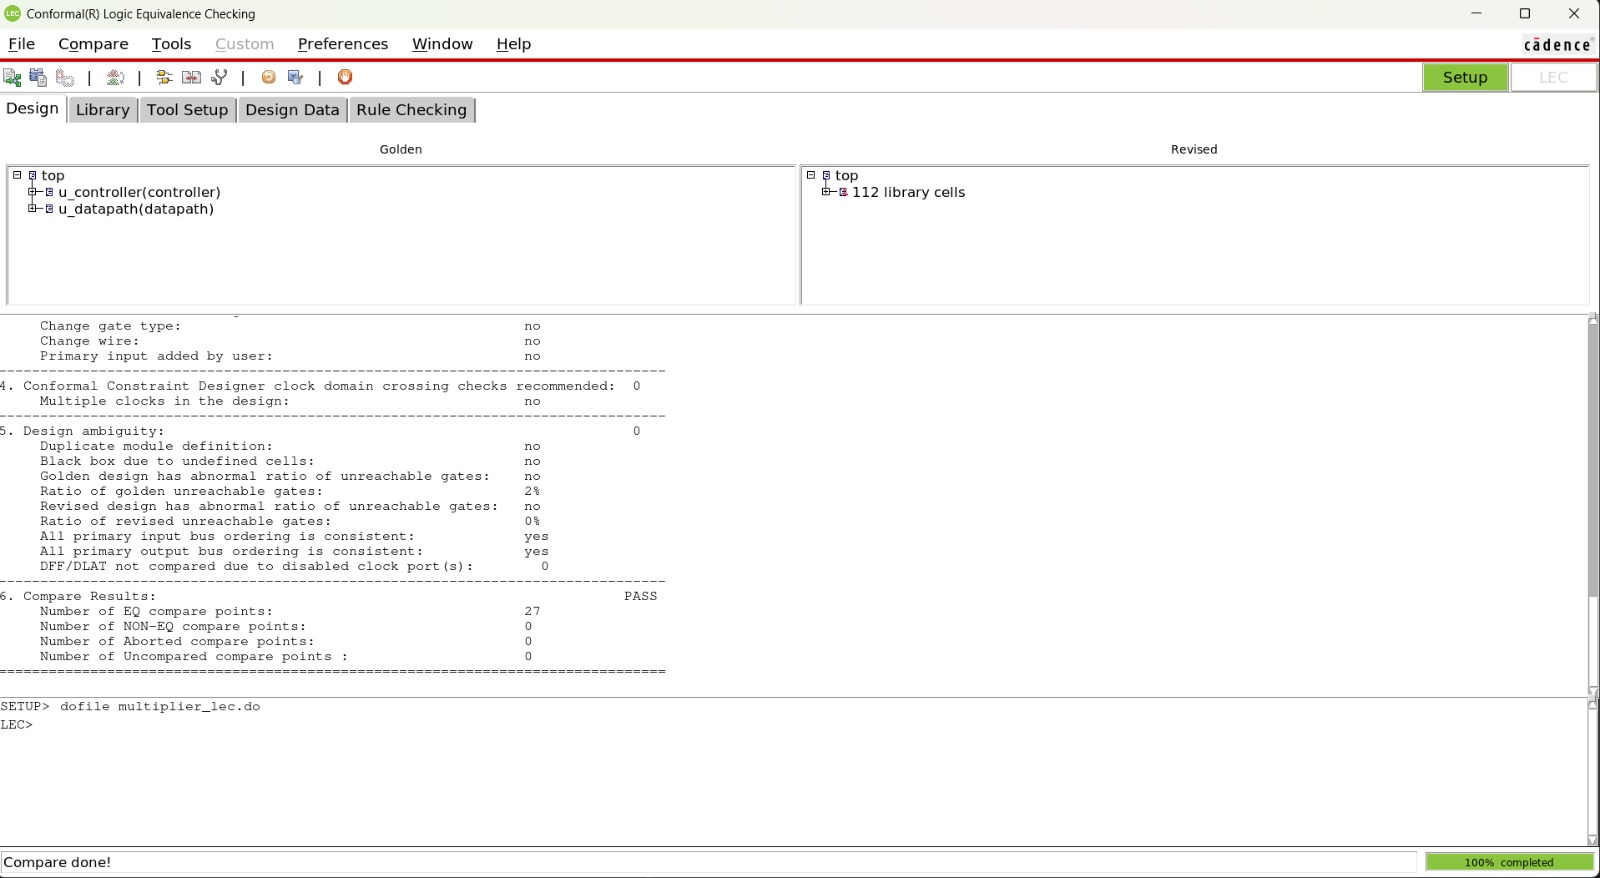
\includegraphics[width=0.9\textwidth]{images/Image_LEC_TASK_1.jpeg}
    \caption{Task 1: LEC PASS with 0 Non-Equivalent points}
\end{figure}

%------------------------------------------------

\section*{Task 2: LEC for Sequential Multiplier with Clock Gating}
\subsection*{Objective}
Enable automatic clock gating insertion during synthesis for power savings, generate a report of deleted sequential elements, and successfully run LEC on the clock-gated netlist by providing the appropriate flattening constraint.

\subsection*{Synthesis Modification}
The Genus synthesis script was modified to include clock gating. The following line was added before reading the Verilog files:
\begin{lstlisting}[language=Tcl]
set_db / .lp_insert_clock_gating true
\end{lstlisting}
Additionally, a report was generated to track the flip-flops that were optimized out by the clock gating logic:
\begin{lstlisting}[language=Tcl]
report_sequential -deleted > work_cg/deleted_flops.rpt
\end{lstlisting}

\subsection*{LEC without Constraint (Demonstration of Failure)}
When running standard LEC on the clock-gated netlist, the verification fails because Conformal cannot map the new clock gating cells (\texttt{RC\_CG\_MOD}) present in the Revised netlist to the Golden RTL. 

\begin{figure}[H]
    \centering
    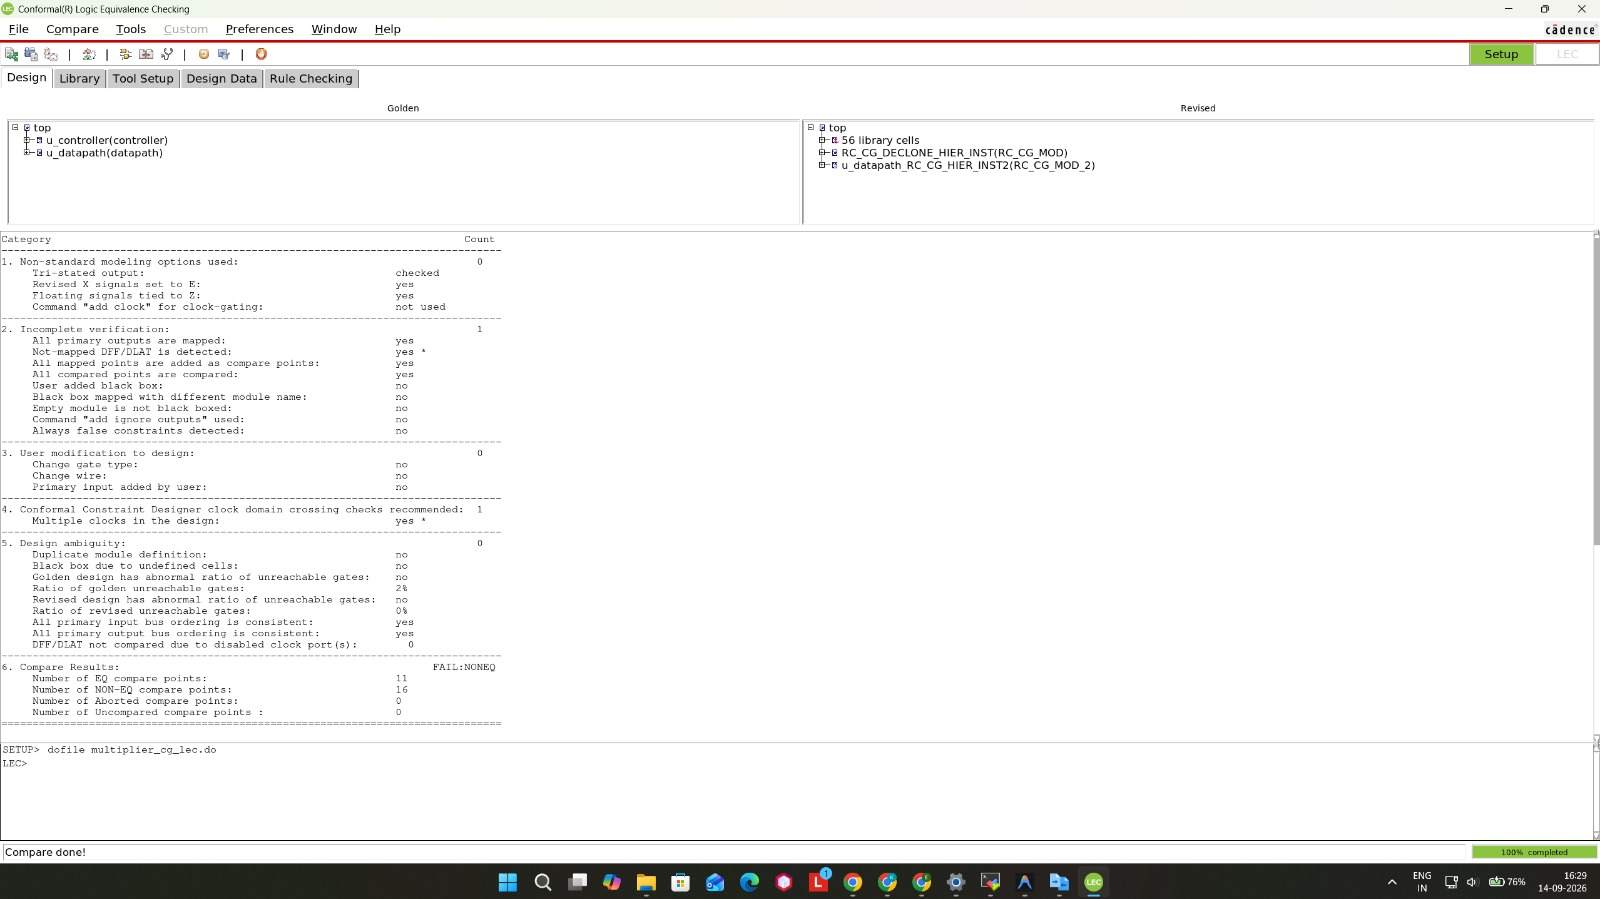
\includegraphics[width=0.9\textwidth]{images/Image_LEC_TASK_2_FAILURE.jpeg}
    \caption{Task 2: LEC Failure (16 Non-Equivalent points) due to unmodeled Clock Gating}
\end{figure}

\subsection*{LEC with Constraint (Fix)}
To instruct the tool to correctly recognize and mathematically flatten the clock gating logic, the following constraint was added to the \texttt{.do} file before switching to LEC mode:
\begin{lstlisting}[language=Tcl]
set flatten model -gated_clock
\end{lstlisting}

After applying this constraint, Conformal was able to correctly compare the logic and verify equivalence.

\begin{figure}[H]
    \centering
    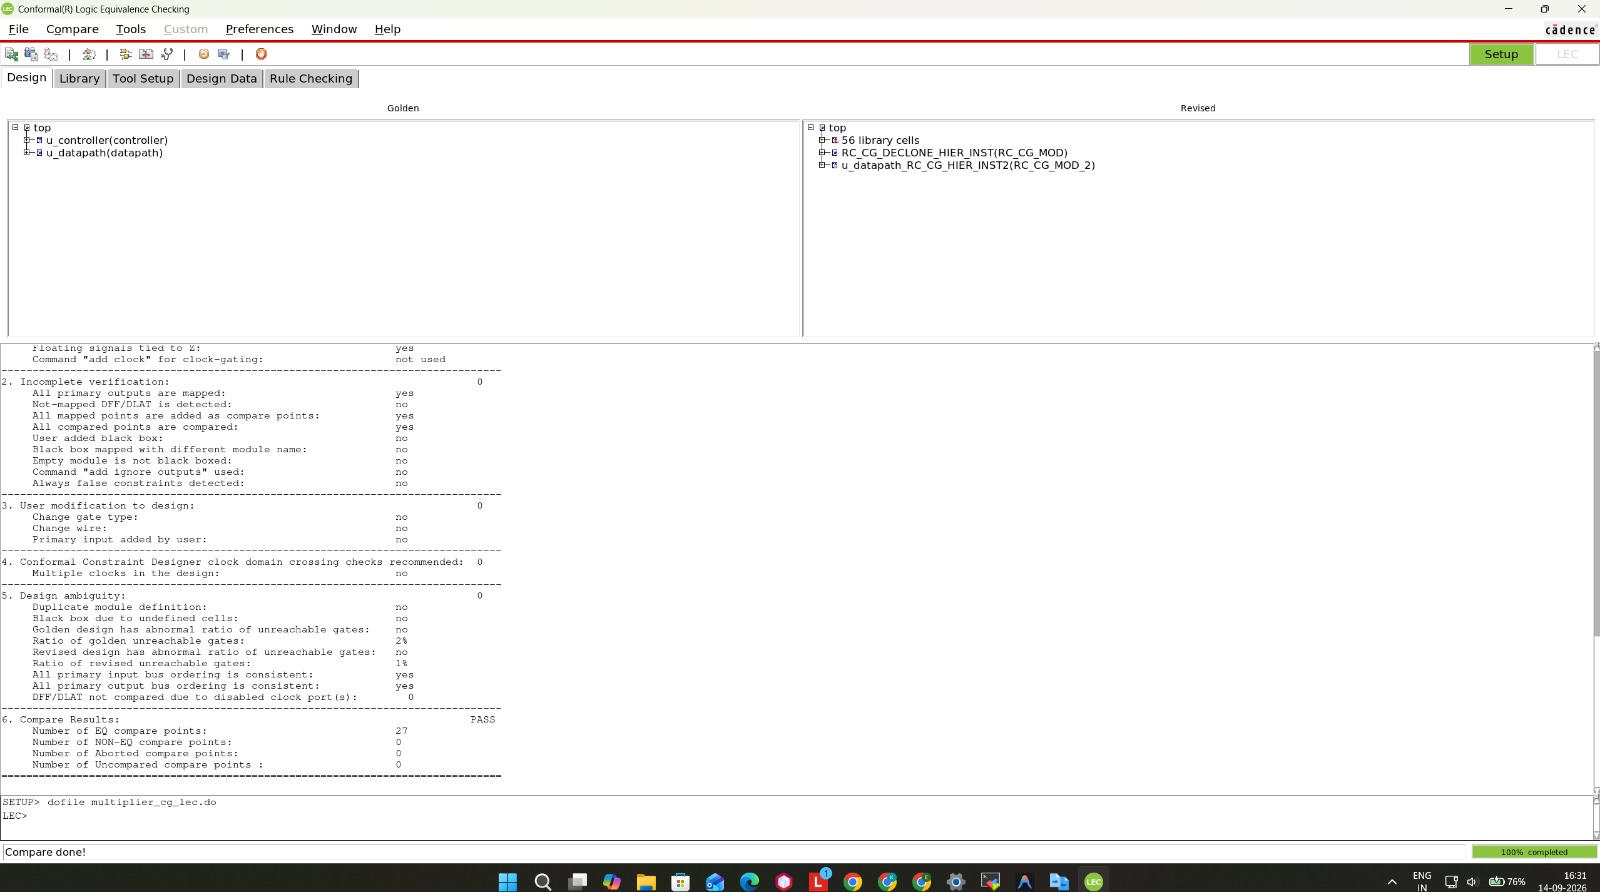
\includegraphics[width=0.9\textwidth]{images/Image_LEC_TASK_2_PASS.jpeg}
    \caption{Task 2: LEC PASS with flattened clock gating models}
\end{figure}

%------------------------------------------------

\section*{Task 3: LEC Run with a Netlist Bug}
\subsection*{Objective}
To intentionally inject a bug into the gate-level netlist and utilize Conformal LEC's graphical debug tools (Mapping Manager and Diagnosis Manager) to identify the root cause of the non-equivalence.

\subsection*{Bug Injection}
A manual edit was made to the \texttt{top\_gates\_buggy.v} netlist. The input to an inverter (\texttt{g1072}) was incorrectly re-routed from \texttt{accumulated\_prod[5]} to \texttt{accumulated\_prod[4]}.

\subsection*{Debugging Process}
Upon running LEC, the tool reported 3 Non-Equivalent compare points. Using the GUI, the following debugging steps were taken:
\begin{enumerate}
    \item Opened the \textbf{Mapping Manager} to filter and identify the specific Non-Equivalent DFFs.
    \item Right-clicked the failing point \texttt{accumulated\_prod\_reg[5]} and selected \textbf{Diagnose}.
    \item In the \textbf{Diagnosis Manager}, Conformal's mathematical solver analyzed the logic cone and correctly identified \texttt{INVX1 g1072} as the primary Error Candidate with a probability of \texttt{1.00}.
    \item The \textbf{Schematics} view was utilized to visually trace the boolean logic error backward from the DFF input, confirming that the Revised logic was pulling from bit \texttt{[4]} while the Golden reference was pulling from bit \texttt{[5]}.
\end{enumerate}

\begin{figure}[H]
    \centering
    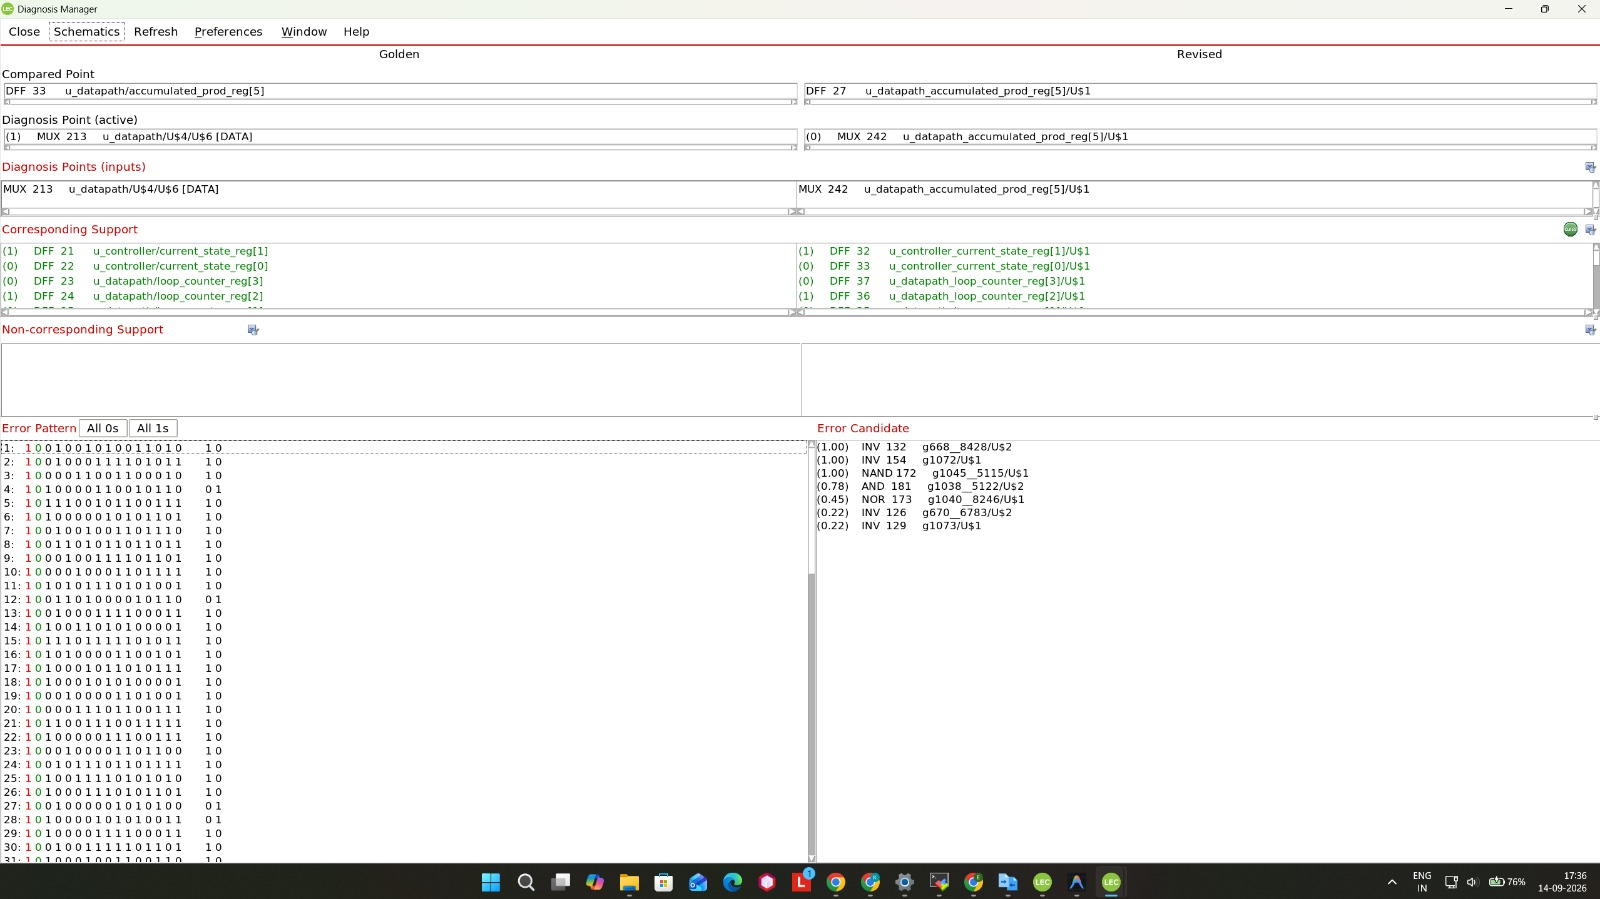
\includegraphics[width=0.9\textwidth]{images/Image_LEC_TASK_3.jpeg}
    \caption{Task 3: Diagnosis Manager identifying g1072 with 1.00 probability}
\end{figure}

\begin{figure}[H]
    \centering
    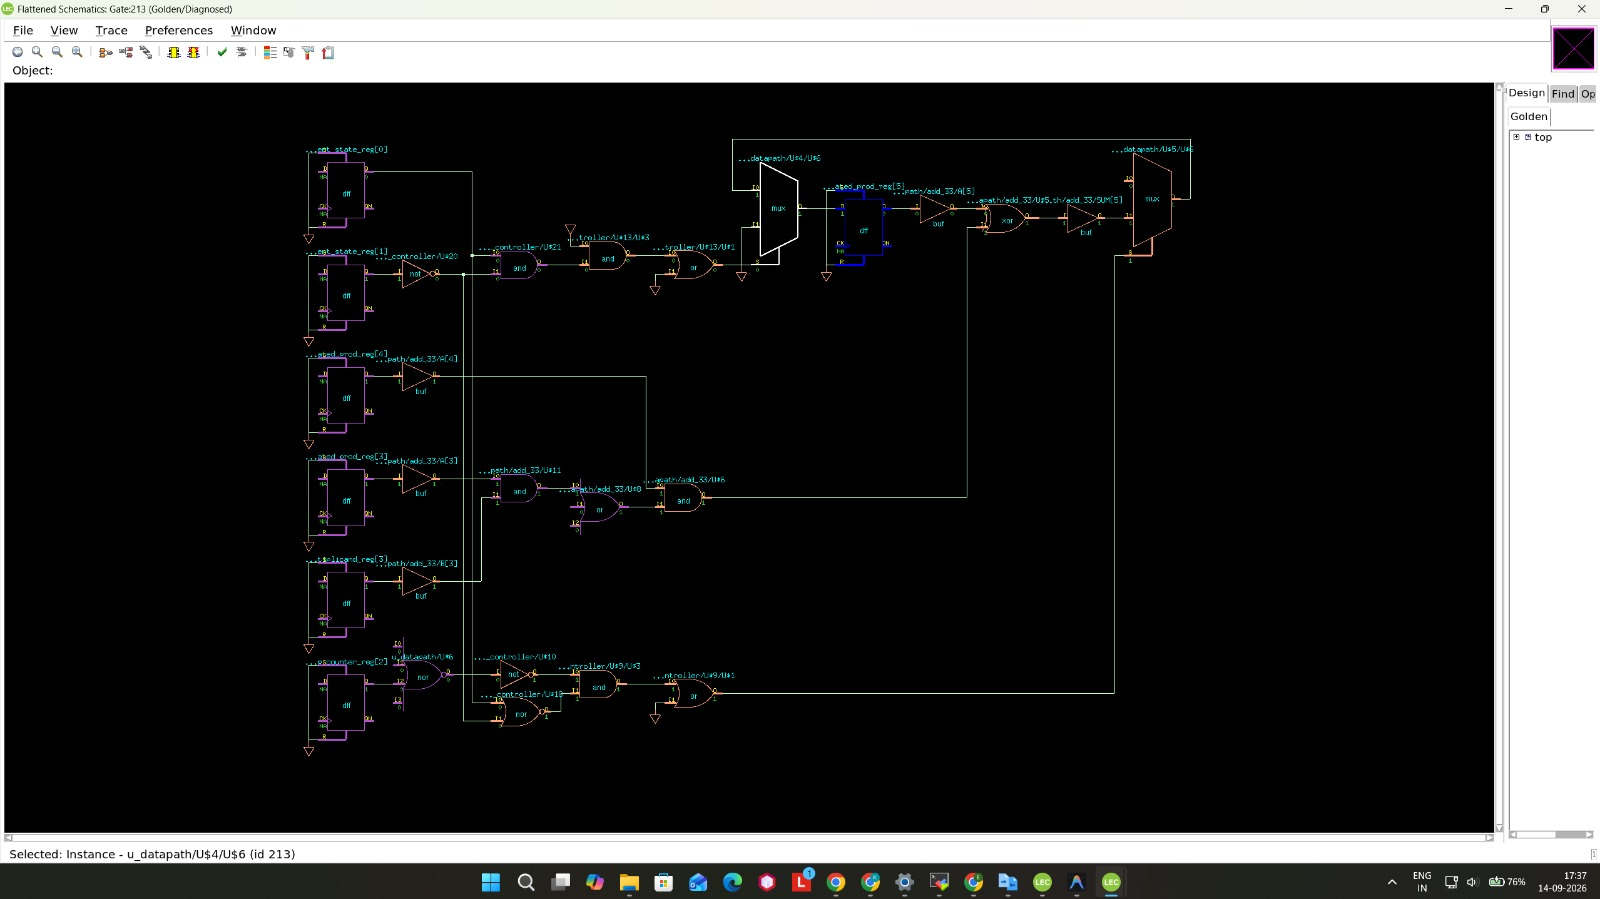
\includegraphics[width=0.9\textwidth]{images/Image_LEC_TASK_3_Golden_Schematic.jpeg}
    \caption{Task 3: Golden flattened schematic at \texttt{accumulated\_prod\_reg[5]}, driven correctly from bit [5]}
\end{figure}

\begin{figure}[H]
    \centering
    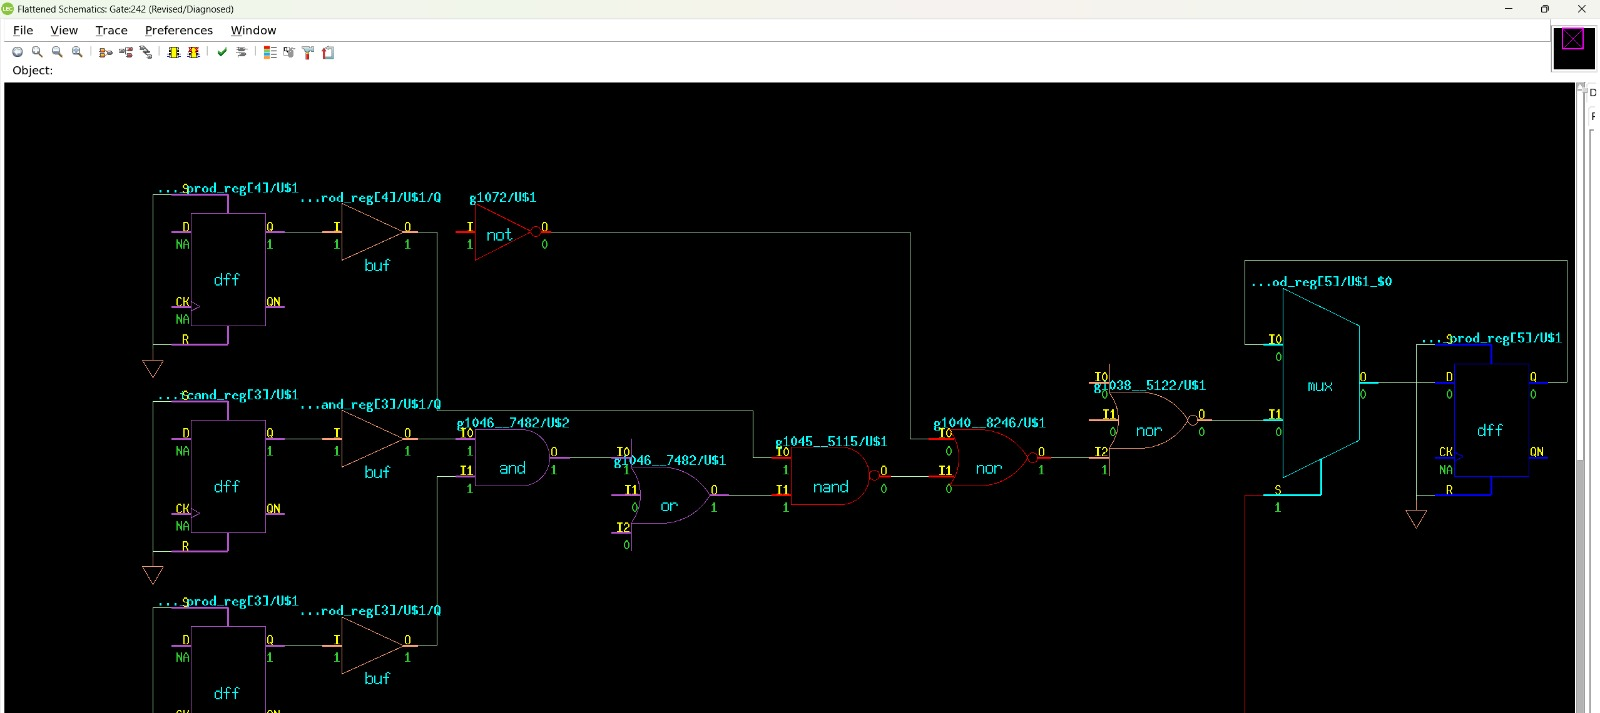
\includegraphics[width=0.9\textwidth]{images/Image_LEC_TASK_3_Revised_Isolating_Fault.jpeg}
    \caption{Task 3: Revised flattened schematic isolating the fault region around \texttt{g1072}}
\end{figure}

\begin{figure}[H]
    \centering
    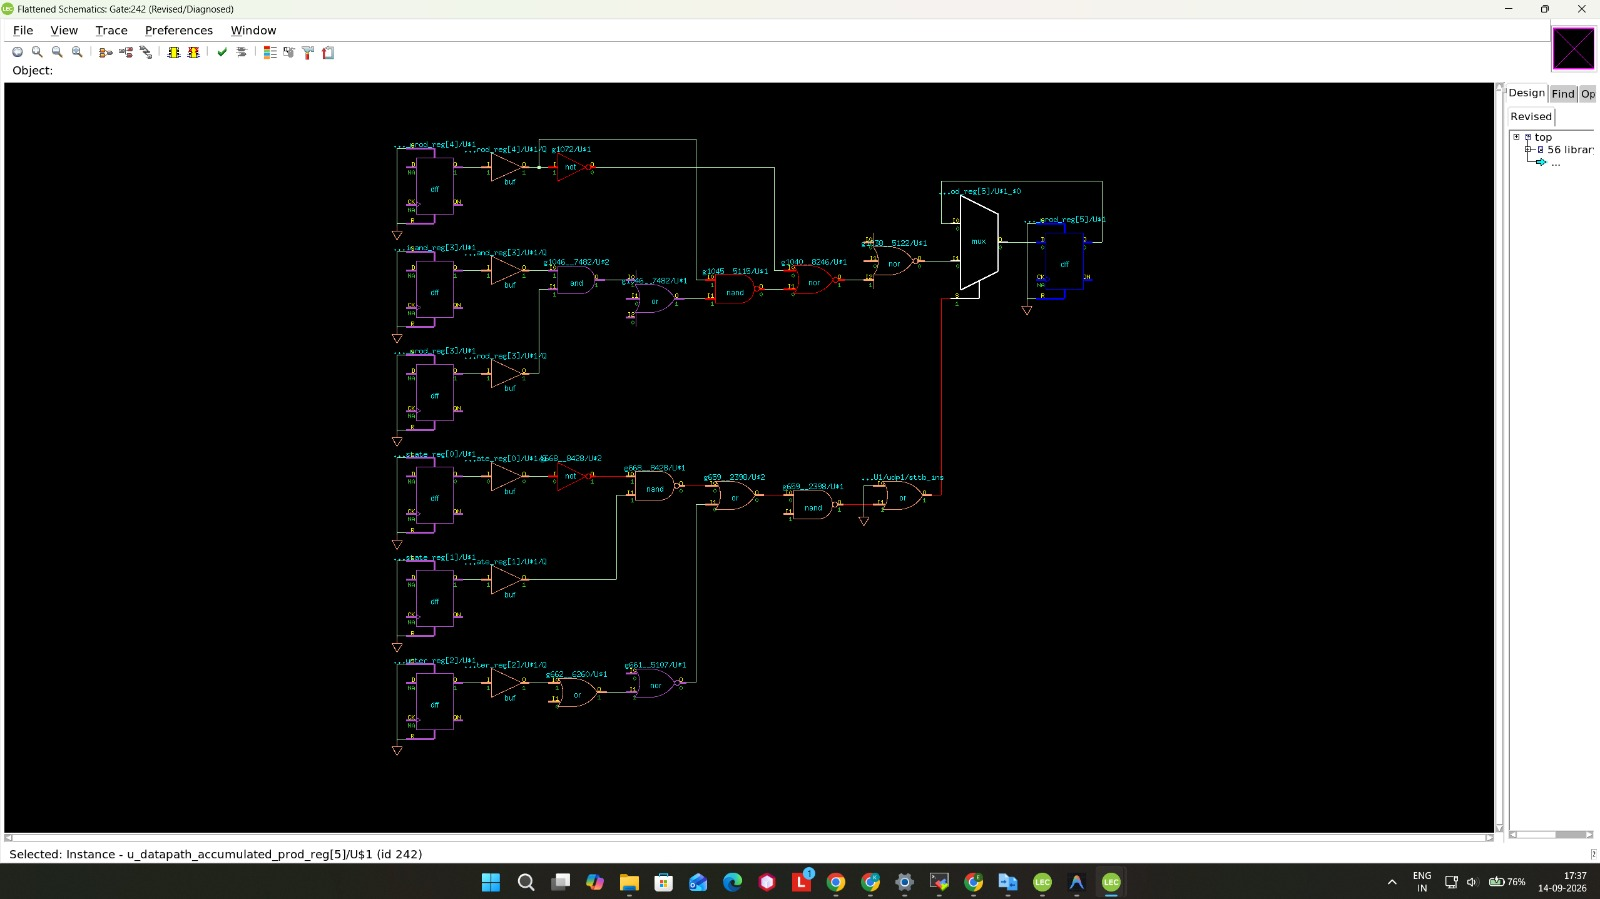
\includegraphics[width=0.9\textwidth]{images/Image_LEC_TASK_3_Revised_Schematic.jpeg}
    \caption{Task 3: Flattened Schematics tracing the error path backward to \texttt{g1072}, showing the incorrect re-route from bit [4]}
\end{figure}

\subsection*{Bug Fix and Verification}
The buggy netlist was corrected by changing the wire mapping back to \texttt{accumulated\_prod[5]}. A final LEC run confirmed the fix.

\begin{figure}[H]
    \centering
    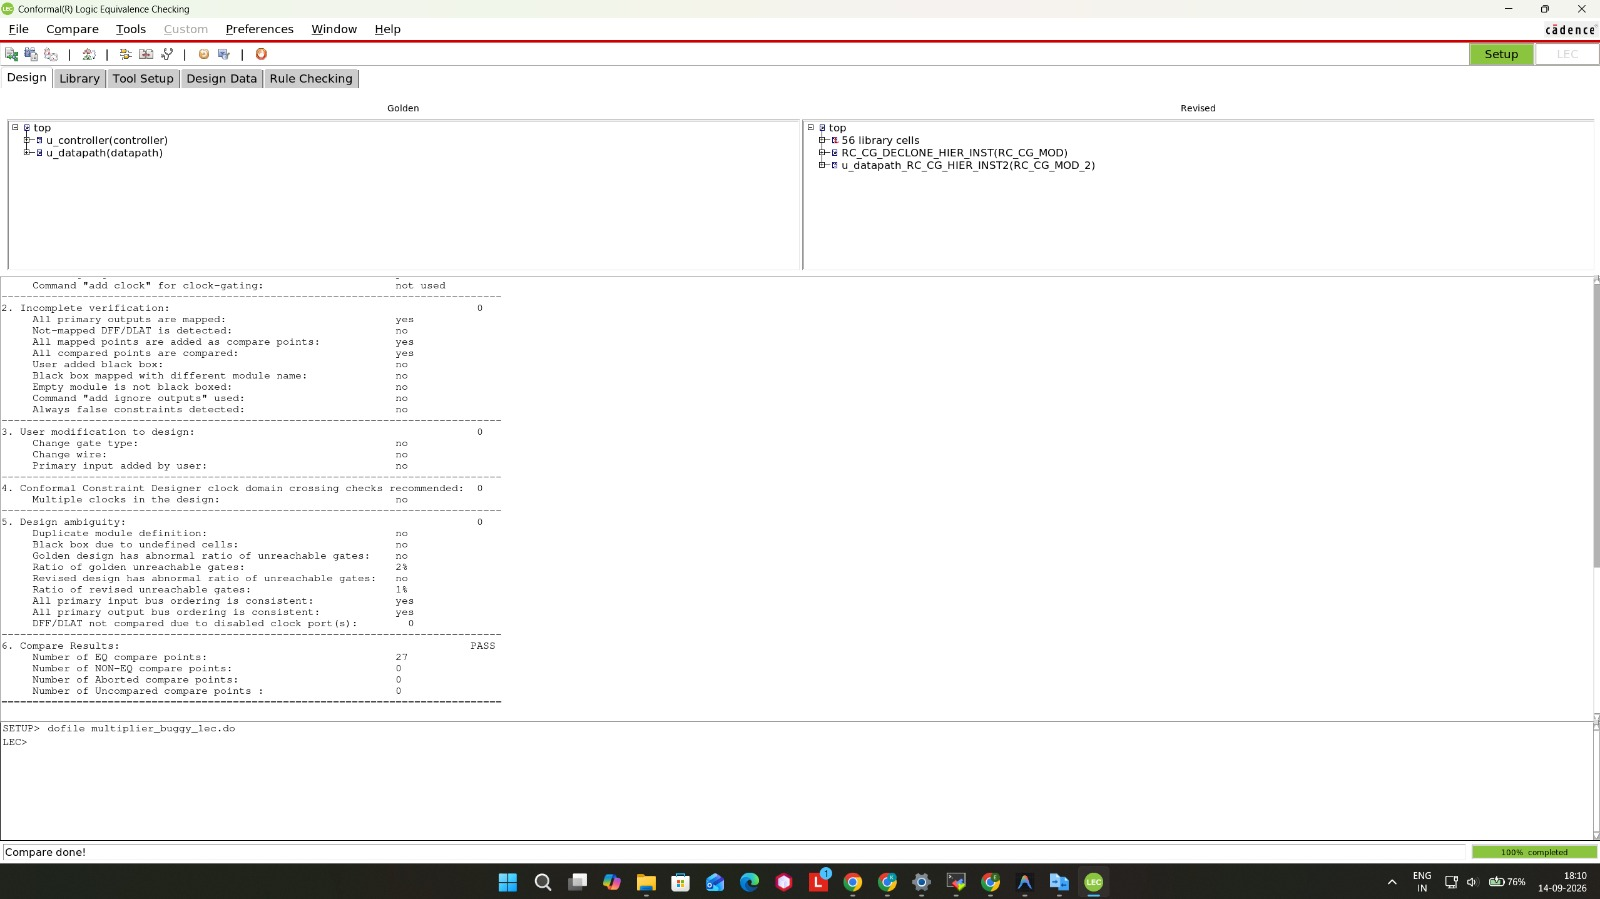
\includegraphics[width=0.9\textwidth]{images/Image_LEC_TASK_3_Pass_Fault_Fixed.jpeg}
    \caption{Task 3: Final LEC PASS after fixing the netlist bug}
\end{figure}

\end{document}
